\documentclass[12pt]{article}

\usepackage[margin=1in]{geometry}
\usepackage{amsmath,amsthm,amssymb}

\usepackage{graphicx}
\graphicspath{ {./assets/} }

\usepackage{algpseudocode}
\usepackage{algorithm}

\usepackage{tikz}

\newcommand{\wip}{\textbf{(WIP) }}
\newcommand{\tba}{\textbf{(TBA) }}

\newcommand{\blah}{\textbf{blah blah blah}}

\newcommand{\dsa}[1]{\textbf{[DSA: #1]}}

\begin{document}

\title{Project 1 — Report}
\author{
  Diogo Antunes\\
  99210
  \and
  Javier María\\
  99240
  \and
  Tomás Silva\\
  98973
}

\maketitle

\section*{Exercise 1}

The first exercise consisted of solving the CNF-SAT $\phi$ formula with the next constraints:

\begin{align}
        & (\lnot p_{1} \vee p_{3} \vee p_{4} \vee p_{5}) \\
        & (\lnot p_{3} \vee p_{4} \vee p_{5}) \\
        & (\lnot p_{1} \vee p_{3} \vee \lnot p_{4}) \\
        & (p_{1} \vee p_{2}) \\
        & (p_{1} \vee \lnot p_{2}) \\
        & (\lnot p_{1} \vee \lnot p_{5}) \\
        & (\lnot p_{3} \vee \lnot p_{4} \vee p_{5})
\end{align}

\vspace{0.5cm}

For this, we used CDCL using 1-UIP (Unit Implication Point) as the conflict analysis strategy.
When going through conflict clauses, if we arrive to a clause with only one literal that is assigned at the current level, we have found the 1-UIP.
We backtrack to the variable with a largest decision level other than the current.

\vspace{0.5cm}

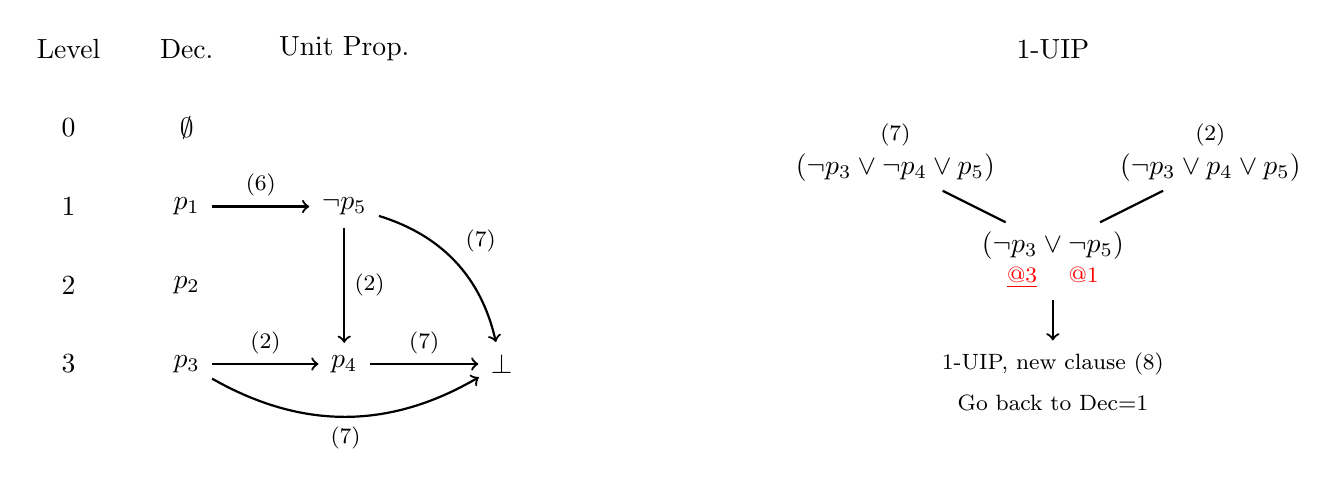
\begin{tikzpicture}[
    every node/.style={anchor=center},
    level/.style={anchor=center},
    decision/.style={anchor=center},
    unit/.style={anchor=center},
    clause/.style={anchor=center},
    arrow/.style={->, thick, shorten >=1pt, shorten <=1pt}
    ]

% Level and Decisions
\node[level] (Level Label) at (0,0) {Level};
\node[level] (Level 0) at (0,-1) {0};
\node[level] (Level 1) at (0,-2) {1};
\node[level] (Level 2) at (0,-3) {2};
\node[level] (Level 3) at (0,-4) {3};

\node[decision] at (1.5,0) {Dec.};
\node[decision] at (1.5,-1) {$\emptyset$};
\node[decision] (p1) at (1.5,-2) {$p_{1}$};
\node[decision] (p2) at (1.5,-3) {$p_{2}$};
\node[decision] (p3) at (1.5,-4) {$p_{3}$};

% Unit Propagation Column
\node[unit] at (3.5,0) {Unit Prop.};

\node[unit] (p5) at (3.5,-2) {$\lnot p_{5}$};
\node[unit] (p4) at (3.5,-4) {$p_{4}$};
\node[unit] (contra) at (5.5, -4) {$\bot$};

% Arrows for Unit Propagation
\draw[arrow] (p1) to node[midway, above] {\footnotesize (6)} (p5);
\draw[arrow] (p3) to node[midway, above] {\footnotesize (2)} (p4);
\draw[arrow] (p5) to node[midway, right] {\footnotesize (2)} (p4);
\draw[arrow] (p4) to node[midway, above] {\footnotesize (7)} (contra);
\draw[arrow, bend right] (p3) to node[midway, below] {\footnotesize (7)} (contra);
\draw[arrow, bend left] (p5) to node[midway, above right] {\footnotesize (7)} (contra);

% Conflict Analysis
\node[clause] (1-UIP Label) at (12.5,0) {1-UIP};
\node[clause] (c7) at (10.5,-1.5) {$(\lnot p_{3} \vee \lnot p_{4} \vee p_{5})$};
\node[above=0.15cm] at (c7) {\footnotesize (7)};
\node[clause] (c2) at (14.5,-1.5) {$(\lnot p_{3} \vee p_{4} \vee p_{5})$};
\node[above=0.15cm] at (c2) {\footnotesize (2)};
\node[clause] (d1) at (12.5,-2.5) {$(\lnot p_{3} \vee \lnot p_{5})$};
\node[below=0.15cm] (levels) at (d1) {\color{red} \footnotesize \underline{@3} \hspace{0.2cm} {@1}};
\node[clause, label={[align=center]below: \footnotesize Go back to Dec=1}] (expl) at (12.5,-4) {\footnotesize 1-UIP, new clause (8)};

% Arrows for conflict analysis
\draw[-, thick] (c7) to (d1);
\draw[-, thick] (c2) to (d1);
\draw[arrow] (levels) to (expl);

\end{tikzpicture}

\vspace{0.5cm}

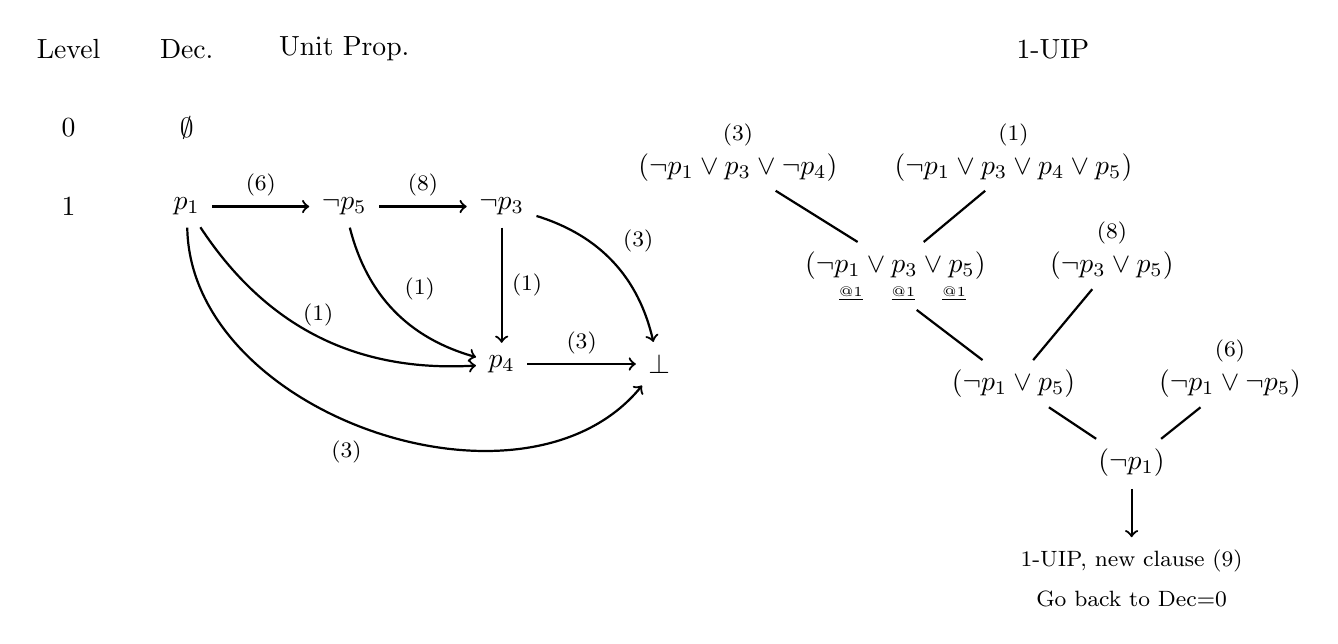
\begin{tikzpicture}[
    every node/.style={anchor=center},
    level/.style={anchor=center},
    decision/.style={anchor=center},
    unit/.style={anchor=center},
    clause/.style={anchor=center},
    arrow/.style={->, thick, shorten >=1pt, shorten <=1pt}
    ]

% Level and Decisions
\node[level] (Level Label) at (0,0) {Level};
\node[level] (Level 0) at (0,-1) {0};
\node[level] (Level 1) at (0,-2) {1};

\node[decision] at (1.5,0) {Dec.};
\node[decision] at (1.5,-1) {$\emptyset$};
\node[decision] (p1) at (1.5,-2) {$p_{1}$};

% Unit Propagation Column
\node[unit] at (3.5,0) {Unit Prop.};

\node[unit] (p5) at (3.5,-2) {$\lnot p_{5}$};
\node[unit] (p3) at (5.5,-2) {$\lnot p_{3}$};
\node[unit] (p4) at (5.5,-4) {$p_{4}$};
\node[unit] (contra) at (7.5, -4) {$\bot$};

% Arrows for Unit Propagation
\draw[arrow] (p1) to node[midway, above] {\footnotesize (6)} (p5);
\draw[arrow] (p5) to node[midway, above] {\footnotesize (8)} (p3);
\draw[arrow, bend right] (p1) to node[midway, above] {\footnotesize (1)} (p4);
\draw[arrow] (p3) to node[midway, right] {\footnotesize (1)} (p4);
\draw[arrow, bend right] (p5) to node[midway, above right] {\footnotesize (1)} (p4);
\draw[arrow, bend left] (p3) to node[midway, above right] {\footnotesize (3)} (contra);
\draw[arrow] (p4) to node[midway, above] {\footnotesize (3)} (contra);
\draw[arrow, bend right=70] (p1) to node[midway, below left] {\footnotesize (3)} (contra);

% Conflict Analysis
\node[clause] (1-UIP Label) at (12.5,0) {1-UIP};
\node[clause] (c3) at (8.5,-1.5) {$(\lnot p_{1} \vee p_{3} \vee \lnot p_{4})$};
\node[above=0.15cm] at (c3) {\footnotesize (3)};
\node[clause] (c1) at (12,-1.5) {$(\lnot p_{1} \vee p_{3} \vee p_{4} \vee p_{5})$};
\node[above=0.15cm] at (c1) {\footnotesize (1)};
\node[clause] (c8) at (13.25, -2.75) {$(\lnot p_{3} \vee p_{5})$};
\node[above=0.15cm] at (c8) {\footnotesize (8)};
\node[clause] (c6) at (14.75, -4.25) {$(\lnot p_{1} \vee \lnot p_{5})$};
\node[above=0.15cm] at (c6) {\footnotesize (6)};
\node[clause] (d1) at (10.5,-2.75) {$(\lnot p_{1} \vee p_{3} \vee p_{5})$};
\node[below=0.15cm] (levels) at (d1) {\tiny \hspace{0.1cm} \underline{@1} \hspace{0.2cm} \underline{@1} \hspace{0.18cm} \underline{@1}};
\node[clause] (d2) at (12,-4.25) {$(\lnot p_{1} \vee p_{5})$};
\node[clause] (d3) at (13.5,-5.25) {$(\lnot p_{1})$};

\node[clause, label={[align=center]below: \footnotesize Go back to Dec=0}] (expl) at (13.5,-6.5) {\footnotesize 1-UIP, new clause (9)};

% Arrows for conflict analysis
\draw[-, thick] (c3) to (d1);
\draw[-, thick] (c1) to (d1);
\draw[-, thick] (levels) to (d2);
\draw[-, thick] (c8) to (d2);
\draw[-, thick] (d2) to (d3);
\draw[-, thick] (c6) to (d3);
\draw[arrow] (d3) to (expl);

\end{tikzpicture}

\vspace{1cm}

\begin{tikzpicture}[
    every node/.style={anchor=center},
    level/.style={anchor=center},
    decision/.style={anchor=center},
    unit/.style={anchor=center},
    clause/.style={anchor=center},
    arrow/.style={->, thick, shorten >=1pt, shorten <=1pt}
    ]

% Level and Decisions
\node[level] (Level Label) at (0,0) {Level};
\node[level] (Level 0) at (0,-1) {0};

\node[decision] at (1.5,0) {Dec.};
\node[decision] (empty) at (1.5,-1) {$\emptyset$};

% Unit Propagation Column
\node[unit] at (3.5,0) {Unit Prop.};

\node[unit] (p1) at (3.5,-1) {$\lnot p_{1}$};
\node[unit] (p2) at (5.5,-1) {$p_{2}$};
\node[unit] (contra) at (5.5, -3) {$\bot$};

% Arrows for Unit Propagation
\draw[arrow] (empty) to node[midway, above] {\footnotesize (9)} (p1);
\draw[arrow] (p1) to node[midway, above] {\footnotesize (4)} (p2);
\draw[arrow, bend right] (p1) to node[midway, above right] {\footnotesize (5)} (contra);
\draw[arrow] (p2) to node[midway, right] {\footnotesize (5)} (contra);

% Conflict Analysis
\node[clause] (1-UIP Label) at (12,0) {1-UIP};
\node[clause] (c5) at (9.5,-1.5) {$(p_{1} \vee \lnot p_{2})$};
\node[above=0.15cm] at (c5) {\footnotesize (5)};
\node[clause] (c4) at (12,-1.5) {$(p_{1} \vee p_{2})$};
\node[above=0.15cm] at (c4) {\footnotesize (4)};
\node[clause] (c9) at (14.5, -1.5) {$(\lnot p_{1})$};
\node[above=0.15cm] at (c9) {\footnotesize (9)};
\node[clause] (d1) at (10.5, -2.75) {$(p_{1})$};
\node[clause] (d2) at (12, -4.25) {$\bot$};

\node[clause] (expl) at (12,-5.5) {\footnotesize Derived $\emptyset \implies$ UNSAT};

% Arrows for conflict analysis
\draw[-, thick] (c5) to (d1);
\draw[-, thick] (c4) to (d1);
\draw[-, thick] (d1) to (d2);
\draw[-, thick] (c9) to (d2);
\draw[arrow] (d2) to (expl);

\end{tikzpicture}

\vspace{1cm}

As we can see from the previous CDCL decision graphs, the formula $\phi$ is unsatisfiable.

\section*{Exercise 2}

% Instructions:
%   - Should include the encoding of the nonogram problem as a SAT problem
% Structure:
% - Two encodings were implemented
% - High-level overview of the encodings
%     - they share some of the structure (of encoding line by line)
%       - explain how this works
%       - In the following sections, we'll only talk about this simplified problem
%     - we have a brute force one that is easier to believe the correctness of but that (has complexity X)
%     - we have a more efficient one that is more complex but also uses less variables (has complexity Y)
%     - from the debugging standpoint, having both implementations proved useful because we were able to use one
% of the implementations to debug the other.
% - ``Brute-force'' approach
%   - One way is to consider all possible combinations
% - Polynomial approach
%   - Intuitively, a brute-force approach doesn't sound right
% - Experimental evaluation
%   - To understand what actually was better, we ran some benchmarks
%   - Show benchmarks, and comment on growth of brute-force approach

Two different encodings for the nonogram problem where implemented and tested.
Both encodings follow the same structure — encoding the entire problem is reduced to encoding a single line with restrictions.
The encoding of the entire problem is just the and of the encodings of all rows and columns.
Let a line be a list of naturals, which denote the gaps that should exist in the line — $l = [g_j, \ldots, g_{j'}]$.
A puzzle is a tuple $\langle H, V\rangle$, where both $H$ and $V$ a list of lines.
The propositional formula that is the encoding of a line $l = [g_j, \ldots, g_{j'}]$ of size $s$ will be denoted $E(l, s)$.
The two approaches will differ precisely on how $E$ is defined.
The encoding of the entire puzzle is

\begin{center}
  $\bigwedge\limits_{l \in H} E(l, |V|) \wedge \bigwedge\limits_{l \in V} E(l, |H|)$
\end{center}

Both approaches will be a variable per cell in the grid (but one of them will have more variables). The variable for cell at row $i$ and column $j$ will be denoted $x_{ij}$.
At a high-level the first encoding uses a ``brute-force'' approach to solving the problem, by considering all possible placements of black regions in a given line.
The second approach tries to avoid this by encoding directly the dependencies between black regions and the rules of the game.
Having both approaches proved useful — the brute-force one was easy to reason about and was used to debug the second approach.
In the following sub-sections, we will look in detail at how each encoding is made.

\subsection*{``Brute-force'' approach}

As hinted at before, the first and simpler approach to encoding the constraints for a single line is to consider all possible placements of segments of the specified sizes on the line.
For instance, if $l = [1, 2]$ for a line of size 5, the possible configurations are the following:

\begin{center}

\begin{tikzpicture}
    % X _ X X _
    \foreach \x in {1,2,...,5} {
        \ifnum\x=1 \filldraw[fill=black] (\x*0.5, 0) rectangle (\x*0.5+0.5, -0.5);
        \else\ifnum\x=3 \filldraw[fill=black] (\x*0.5, 0) rectangle (\x*0.5+0.5, -0.5);
        \else\ifnum\x=4 \filldraw[fill=black] (\x*0.5, 0) rectangle (\x*0.5+0.5, -0.5);
        \else \draw (\x*0.5, 0) rectangle (\x*0.5+0.5, -0.5);
        \fi\fi\fi
    }

    % X _ _ X X
    \begin{scope}[shift={(3.5, 0)}]
    \foreach \x in {1,2,...,5} {
        \ifnum\x=1 \filldraw[fill=black] (\x*0.5, 0) rectangle (\x*0.5+0.5, -0.5);
        \else\ifnum\x=4 \filldraw[fill=black] (\x*0.5, 0) rectangle (\x*0.5+0.5, -0.5);
        \else\ifnum\x=5 \filldraw[fill=black] (\x*0.5, 0) rectangle (\x*0.5+0.5, -0.5);
        \else \draw (\x*0.5, 0) rectangle (\x*0.5+0.5, -0.5);
        \fi\fi\fi
    }
    \end{scope}

    % _ X _ X X
    \begin{scope}[shift={(7, 0)}]
    \foreach \x in {1,2,...,5} {
        \ifnum\x=2 \filldraw[fill=black] (\x*0.5, 0) rectangle (\x*0.5+0.5, -0.5);
        \else\ifnum\x=4 \filldraw[fill=black] (\x*0.5, 0) rectangle (\x*0.5+0.5, -0.5);
        \else\ifnum\x=5 \filldraw[fill=black] (\x*0.5, 0) rectangle (\x*0.5+0.5, -0.5);
        \else \draw (\x*0.5, 0) rectangle (\x*0.5+0.5, -0.5);
        \fi\fi\fi
    }
    \end{scope}
\end{tikzpicture}
\end{center}

\noindent Before defining the function, we need to define the minimum and maximum start positions for a given gap.

\noindent Given the constraints of the problem, a given gap cannot start at any position in the line.
To avoid considering positions which are impossible regardless of the other constraints that might exist, a minimum and maximum start positions are defined.
The miminum start position for gap $gaps_i$ is defined as $minStart(gaps_i) = \sum_{j = 0}^{i-1}(gaps_{j}+ 1)$. Similarly, the maximum start position for a gap $i$ is $maxStart(gaps_i) = size - g - \sum_{j=i+1}^{size}(gaps_{j} + 1)$.

In general, the list of all possible starts is given by the following function:

\begin{algorithm}
\caption{Function to compute all possible start configurations}\label{alg:allPossible}
\begin{algorithmic}
\Function{AllPossible}{$gaps$, $size$}
  \If{len ($gaps$) = 1}
    \State\Return$[ [i]: 0 \le i \le size - gaps_0]$
  \Else
    \State$all = []$
    \For{$i = 0$ to $size - gaps_0$}
      \State$o = start + g + 1$ \Comment{Offset of remaining starts}
      \ForAll{$pos \in AllPossible(gaps[1..], size - o)$}
          \State $all.append([i] + [p + o: p \in pos])$
      \EndFor
    \EndFor
    \State \Return $all$
  \EndIf
\EndFunction
\end{algorithmic}
\end{algorithm}

As can be seen, a start configuration is a list of integers that mark where each gap should start.
Given a configuration and the list of gaps, the set of filled positions is $filled(starts, gaps) = \{j\ |\ \exists i: starts_i \le j \le starts_i + gaps_i\}$.

A single start configuration can be encoded as follows:

\begin{center}
  $E(starts, gaps) = \bigwedge\limits_{i \in filled(starts, gaps)}x_i \wedge \bigwedge\limits_{i \notin filled(starts, gaps)} \neg x_i$
\end{center}

\noindent Given the list of all possible starts, the encoding is quite straightforward:

\begin{center}
  $E(l, s) = \bigvee_{starts \in AllPossible(l, s)} E(starts, l)$
\end{center}

\noindent As can be seen, the complexity of this approach is rather bad. As the number of gaps grows, the number of possible combinations is exponential. In particular, if there are $k$ gaps in a line of size $s$, the number of combinations is $\mathcal{O}(s^k)$ possibilities.\footnote{This is a bit of an overestimation, because we only place gaps between the minimum and maximum positions}

\subsection*{Polynomial approach}

This approach attempts to encode not what are the possible combinations that result from the restrictions of the puzzle but the actual rules and restrictions of the nonogram game.
For this, we require an extra set of variables — $c_{ij}$ (note that when solving the entire puzzle, conditions for different lines are distinct and so must be given distinct names).
For a given line, $c_{ij}$ is intended to mean the gap $i$ was already placed when one gets to position $j$ (when considered from left to right). An ``ghost'' position at the end is considered for convinience (i.e. $c_{ij}$ exists for $j = size$ as well).
For instance, consider the following example.

\begin{center}
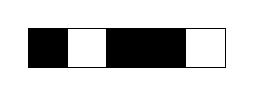
\begin{tikzpicture}
    % X _ X X _
    \foreach \x in {1,2,...,5} {
        \ifnum\x=1 \filldraw[fill=black] (\x*0.5, 0) rectangle (\x*0.5+0.5, -0.5);
        \else\ifnum\x=3 \filldraw[fill=black] (\x*0.5, 0) rectangle (\x*0.5+0.5, -0.5);
        \else\ifnum\x=4 \filldraw[fill=black] (\x*0.5, 0) rectangle (\x*0.5+0.5, -0.5);
        \else \draw (\x*0.5, 0) rectangle (\x*0.5+0.5, -0.5);
        \fi\fi\fi
    }
\end{tikzpicture}
\end{center}

\noindent The condition variables will take the following values

\begin{align*}
c_{00} &= F & c_{01} &= T & c_{02} &= T & c_{03} &= T & c_{04} &= T & c_{05} &= T \\
c_{10} &= F & c_{11} &= F & c_{12} &= F & c_{13} &= F & c_{14} &= T & c_{15} &= T
\end{align*}

\noindent Having these extra variables will allow us to encode all the requirements we need. Unlike the previous approach we need to encode several rules, not just the solution.

\begin{enumerate}
  \item If the $i$-th gap starts at at position $s$, then we need to ensure that the following $gaps_i - 1$ positions are filled and that the next position is empty.
      Additionally, we need to ensure that the we haven't starts completing this gap and that the previous one has already been completed -- which can be done using the constraint variables.
      Two exceptions to this rule are required.
      The first gap does not require the previous gap to be completed.
      In last gap not only the cell after, but all cells up to the end (possibily zero) must be empty.
      Only the general rule is presented:
      \begin{center}
        $\forall i, s: \neg c_{i}_{(s+gaps_i-1)} \wedge c_{(i-1)}_{(start-1)} \wedge x_s \implies c_{i}_{(s+gaps_i)} \wedge \bigwedge_{k=s}^{s+gaps_i-1} x_k \wedge \neg x_{s+gaps_i}$
      \end{center}


    \item The previous rule described how to complete the gap, but doesn't require that that is the only way to do that.
          For that reason, we need to require that if a gap is complete by a given cell, then it was either just completed (which can be checked by looking at the values of $x$) or the previuos one was completed.
          \begin{center}
            $\forall i, j \ne 0: c_{i}_{j} \implies c_{i}_{(j-1)} \vee \bigwedge_{k=j-gaps_i}^{j-1} x_k$
          \end{center}

          For cells where the gap could never have started, a tigther condition can be specified
          \begin{center}
            $\forall i, j \ne 0: c_{i}_{j} \implies c_{i}_{(j-1)}$
          \end{center}

  \item We also specified that for a gap to start completing, then the previous should have completed, but again we didn't specify that if a gap hasn't completed, the next hasn't completed as well. In fact, we can be more strict, if a gap hasn't completed by a position $j$, then the following won't complete at $j$, nor at any position before $j+nextGap$.

  \begin{center}
    $\forall i \ne |gaps|-1, 0 \le k < maxStart(gaps_i): \neg c_i_{(k+gaps_i)} \implies \bigwedge_k^{k+gaps_i+1} \neg c_{(i+1)}_{(j + gaps_{i+1})}$
  \end{center}

  \item If a given gap is completed by position $s$, then it is also completed at position $s+1$.
  \begin{center}
    $\forall i, 0 \le s \le size: (c_i_s \implies c_{(i+1)}_s) $
  \end{center}

  \item Before a gap reaches the minimum position where it can be completed, the completion variables must be false. This represents the start condition.
  \begin{center}
    $\forall i, 0 \le s \le minStart(gaps_i)+gaps_i: \neg c_i_{size}$
  \end{center}

  \item At the end everything should be completed.

  \begin{center}
    $\forall i, c_i_{size}$
  \end{center}
\end{enumerate}

As can be seen, at no point all possible combinations are considered. For that reason, at most a polynomial amount of restrictions are added.

\subsection*{Evaluation}

In this section we compare the two approaches described previously.
For that a puzzle generator was implemented. The puzzle size was set to be the sum of the number of rows and columns. For each puzzle size, a puzzle is generated and then both approaches are used to solve it -- both the initialization time and the SAT solving time are measured. This is repeated 100 times. The results can be seen in Figure~\ref{fig:bench}.

\begin{figure}[H]
  \includegraphics[scale=0.5]{bench.png}
  \centering
  \caption{Execution time for both algorithms proposed}
  \label{fig:bench}
\end{figure}

As can be seen, the polynomial approach is slower for small puzzles, but as soon as the puzzle size reaches 25 it becomes the faster approach.

Additionally, the percentage of time was analysed — the results are in Figure~\ref{fig:util}

As expected, the initialization time dominates the solving time, especially for smaller problems.

\begin{figure}[H]
  \includegraphics[scale=0.5]{util.png}
  \centering
  \caption{Percentage of time spent in SAT solver}
  \label{fig:bench}
\end{figure}

% TODO: say more stuff

% \listoffigures

\end{document}
